\section{Problem Analysis \& Requirements Elicitation}
\label{sec:problem_analysis}

\subsection{Problem Statement}
\label{subsec:problem_statement}

\subsubsection{Domain Context}
Digital comic consumption---spanning South Korean \textit{Webtoons} (vertical long-strip format), Japanese \textit{Manga} (paginated right-to-left or left-to-right format), and Chinese \textit{Manhua}---has grown into one of the most dominant mobile entertainment habits among students and young professionals. Unlike desktop media consumption, mobile comic reading occurs across highly fragmented micro-sessions throughout the day: during lunch breaks between university lectures or office shifts, while commuting on public transit (buses, metro trains, ride-hailing vehicles), during short idle intervals, and during late-night wind-down routines before sleep ($22\text{:}00\text{--}00\text{:}30$).

\subsubsection{Core User Pain Points in Existing Platforms}
Despite massive demand, current mobile comic readers and unofficial aggregator websites suffer from seven severe technical and user-experience deficiencies identified through our domain investigation and user elicitation:

\begin{enumerate}[label=\textbf{Pain Point \arabic*:}, wide=0pt, leftmargin=1.6em]
    \item \textbf{Intrusive and Harmful Advertisements:} Free comic applications and pirated web aggregators aggressively inject auto-playing full-screen video advertisements with unmuted audio, persistent bottom/top banners that obscure artwork panels, and deceptive pop-up redirects to illicit gambling or malware sites. This shatters narrative immersion and wastes mobile cellular data.
    \item \textbf{Language Barriers and Unfinished Scanlations:} Readers frequently encounter situations where an international series has released dozens of new chapters in its raw or English edition, whereas community Vietnamese translation (\textit{scanlation}) groups have either fallen months behind or abandoned (\textit{dropped}) the project entirely.
    \item \textbf{Fragmented Catalogs and Inability to Search by Image:} Readers are forced to install three to four separate applications simultaneously to follow their favourite series. Furthermore, when users encounter a visually striking comic panel or screenshot on social media (\textit{TikTok, Facebook, Threads}) without a title credit, existing mobile apps offer no visual reverse-search mechanism to identify the series.
    \item \textbf{Poor Offline Resilience and Restrictive Paywalls:} Unstable 4G/5G cellular coverage during transit causes conventional online readers to freeze indefinitely on spinning loading indicators. Meanwhile, commercial apps either prohibit local chapter downloads or lock offline caching behind expensive VIP subscriptions and expiring 30-day rental coins, while unmanaged image caches silently bloat device storage.
    \item \textbf{Sub-optimal Scrolling Performance (Frame Drops):} Poorly engineered readers decode and retain all high-resolution images of a 40--60 page Webtoon chapter in memory simultaneously, triggering severe UI jank, dropped frames ($< 30\text{ FPS}$), and Out-Of-Memory (OOM) crashes during rapid vertical scrolling.
    \item \textbf{Monotonous Single-Sense Reading Experience:} Traditional digital comic reading is strictly static and silent, lacking subtle, genre-matched instrumental background audio (\textit{ambient rain, soft piano, lo-fi beats, or orchestral tension}) that resonates with the emotional atmosphere of the narrative without forcing the user to manually juggle a separate music streaming app in the background.
    \item \textbf{Lack of Cross-Device Cloud Synchronisation:} When users switch smartphones, read across a phone and tablet, or reinstall an application, they routinely lose their entire bookmarked library and exact page-level reading progress due to the absence of a secure cloud account synchronisation layer.
\end{enumerate}

\subsection{Stakeholder Analysis}
\label{subsec:stakeholders}

Table~\ref{tab:stakeholders} identifies the primary, internal, platform, external, and indirect stakeholders of the \textbf{Naomi} ecosystem along with their roles and technical expectations.

\begin{table}[H]
\centering
\caption{Stakeholder classification, roles, and expectations for the Naomi ecosystem.}
\label{tab:stakeholders}
\footnotesize
\renewcommand{\arraystretch}{1.25}
\begin{tabularx}{\textwidth}{L{3.2cm} C{2.2cm} Y}
\toprule
\rowcolor{tablehead}
\textbf{Stakeholder} & \textbf{Category} & \textbf{Role \& Expectations for the Naomi System} \\
\midrule
\textbf{End-Users (Mobile Comic Readers)} & Primary & Expect a $100\%$ ad-free reading environment, personal cloud account synchronisation, buttery-smooth $60\text{ FPS}$ vertical/horizontal rendering, automatic page-level progress tracking, genre-matched instrumental ambient audio, free 1-tap offline reading, and intelligent utilities (in-place AI translation, zero-permission visual search). \\
\rowcolor{tablerow}
\textbf{Development Team (Engineering)} & Internal & Responsible for architecting the system using strict Clean Architecture and BLoC state management, enforcing bounded LRU disk caching ($\le 500\text{ MB}$) to prevent OOM crashes, integrating REST/BaaS APIs cleanly, and maintaining high unit-testability for Assignment 02. \\
\textbf{Cloud Backend Provider (Supabase)} & Platform & Provides enterprise-grade JWT authentication (\texttt{Supabase Auth}), cloud relational persistence (\texttt{PostgreSQL} with Row-Level Security), and object storage (\texttt{Supabase Storage}) for user profiles, bookmarks, reading history, and instrumental audio streams. \\
\rowcolor{tablerow}
\textbf{External Content API (MangaDex API v5)} & External & Supplies open global comic metadata and decentralised \texttt{MangaDex@Home} CDN page delivery; requires the client application to strictly respect rate limits ($5\text{ req/s}$), exponential backoff, and caching headers. \\
\textbf{Community Scanlation Groups} & Indirect Partner & Expect their translated chapters and credits to be preserved intact and delivered within a strictly non-commercial, ad-free reader without unauthorized paywall monetisation. \\
\bottomrule
\end{tabularx}
\end{table}

\subsection{User Personas}
\label{subsec:personas}

Grounded directly in our empirical survey responses and qualitative behavioural interviews (Section~\ref{subsec:elicitation}), three representative User Personas were constructed to guide feature prioritisation and UI/UX decisions.

\subsubsection{Persona 1: Nguyen Tuan Kiet --- ``The Late-Night Immersionist''}
\textit{Represents late-night readers ($22\text{:}30\text{--}00\text{:}30$, Survey Q1), highly receptive to genre-matched background audio (Survey Q3 \& Q4), and deeply frustrated by loud video ads and scrolling lag (Survey Q2).}
\begin{itemize}
    \item \textbf{Demographics \& Device:} 21-year-old third-year Information Technology undergraduate; uses a Xiaomi Redmi Note 12 (Android 13, $120\text{ Hz}$ AMOLED display).
    \item \textbf{Reading Context \& Psychology:} Reads in bed every night between $22\text{:}30$ and $00\text{:}30$. For Kiet, late-night reading is not casual time-killing but an emotional decompression and healing ritual after intense coding sessions. He frequently opens Spotify in the background to play lo-fi or rain tracks while reading because gentle piano or rainfall deepens emotional scenes, whereas rhythmic instrumental tracks heighten action sequences.
    \item \textbf{Core Frustrations:}
    \begin{enumerate}[label=(\alph*)]
        \item \textit{Immersion-shattering video ads:} Unmuted gambling video ads suddenly blasting at maximum volume at midnight, startling him awake and ruining his sleep.
        \item \textit{Scrolling stutter:} Frame drops when scrolling through 40--50 high-resolution Webtoon strips.
        \item \textit{Battery \& thermal drain:} Running Spotify alongside a heavy comic app causes his phone to overheat and drain battery rapidly.
    \end{enumerate}
    \item \textbf{Goals with Naomi:} A $100\%$ ad-free reader with an eye-soothing AMOLED Dark Mode (\texttt{\#111116}), built-in instrumental ambient audio automatically matched to the comic's genre with a minimal volume slider, and seamless toggling between $60\text{ FPS}$ vertical Webtoon scrolling and horizontal Manga page-flipping.
\end{itemize}

\subsubsection{Persona 2: Tran Phuong Thao --- ``The On-The-Go \& Social Hunter''}
\textit{Represents opportunistic daytime readers ($50\%$ in Survey Q1), frustrated by cellular dropouts and paywalled offline modes (Survey Q2), and eager for visual image search (Survey Q5).}
\begin{itemize}
    \item \textbf{Demographics \& Device:} 20-year-old second-year Multimedia Communications student in Ho Chi Minh City; uses a Samsung Galaxy A54 (Android 14, capped monthly 4G data plan).
    \item \textbf{Reading Context \& Psychology:} Reads during 10--15 minute breaks between classes or while commuting on buses and ride-hailing bikes. Actively browses TikTok, Facebook, and Threads, where she frequently saves screenshots of aesthetically striking comic panels that lack title captions.
    \item \textbf{Core Frustrations:}
    \begin{enumerate}[label=(\alph*)]
        \item \textit{Dead-ends when searching by image:} Having to post uncredited screenshots in community groups and wait hours for someone to identify the comic title.
        \item \textit{Cellular network freezes:} Online apps freezing on an endless loading spinner whenever the bus passes through weak 4G reception zones.
        \item \textit{Paywalled offline downloads:} Commercial apps locking offline chapter downloads behind paid VIP tiers or expiring coins.
    \end{enumerate}
    \item \textbf{Goals with Naomi:} Zero-permission Visual Search via the OS Photo Picker to identify comics from saved screenshots instantly, free 1-tap offline chapter downloading over home Wi-Fi for lag-free transit reading, and a clean two-category Personal Library (\textit{Favorites} and \textit{Offline Reading}).
\end{itemize}

\subsubsection{Persona 3: Le Minh Duc --- ``The Fast-Paced Early Reader''}
\textit{Represents lunch-break readers (Survey Q1) who follow multiple ongoing series, encounter untranslated latest chapters (Survey Q2), and demand in-place AI translation ($100\%$ in Survey Q5) and exact page-level history ($75\%$ in Survey Q5).}
\begin{itemize}
    \item \textbf{Demographics \& Device:} 23-year-old junior software engineer working in Hanoi; uses a Google Pixel 7 (Android 14).
    \item \textbf{Reading Context \& Psychology:} Reads during his office lunch break ($11\text{:}45\text{--}12\text{:}45$) or after overtime. Follows 5--7 ongoing action/fantasy series simultaneously and wants to read newly released chapters immediately upon international publication.
    \item \textbf{Core Frustrations:}
    \begin{enumerate}[label=(\alph*)]
        \item \textit{Abandoned translations:} When an international series reaches Chapter 150 but local scanlation groups stop at Chapter 100, switching back and forth between the comic app and Google Translate destroys reading flow.
        \item \textit{Lost reading position:} Abruptly closing the app when work resumes and returning the next day only to find the app forgot which page he was on within a 50-page chapter.
    \end{enumerate}
    \item \textbf{Goals with Naomi:} Automatic page-level reading history synced to a prominent \textit{Continue Reading} hero card on the Home screen, in-place AI chapter translation (\texttt{FR-12}), and genre-based recommendations upon finishing a chapter.
\end{itemize}

\subsection{Competitor Analysis}
\label{subsec:competitor_analysis}

To position \textbf{Naomi} objectively within the mobile entertainment market, we conducted a comparative evaluation against the two dominant market leaders representing distinct segments: \textbf{LINE Webtoon} (the leading global official platform) and \textbf{MangaToon} (a widely used commercial aggregator in Vietnam). Table~\ref{tab:competitors} synthesises the technical and experiential comparison.

\begin{table}[H]
\centering
\caption{Quantitative and qualitative competitor comparison across key mobile comic reader dimensions.}
\label{tab:competitors}
\footnotesize
\renewcommand{\arraystretch}{1.25}
\begin{tabularx}{\textwidth}{L{3.5cm} L{3.6cm} L{3.6cm} Y}
\toprule
\rowcolor{tablehead}
\textbf{Evaluation Dimension} & \textbf{LINE Webtoon (Global)} & \textbf{MangaToon (Vietnam)} & \textbf{Naomi (Proposed System)} \\
\midrule
\textbf{Advertisement Intrusiveness} & Moderate (mandatory video ads for Daily Pass, promotional pop-ups) & \textbf{Severe} (pop-up banners, gambling redirects, panel-obscuring ads) & \textbf{100\% Ad-Free} (zero ad SDKs, zero pop-ups or paywalls) \\
\rowcolor{tablerow}
\textbf{Interactive Ambient Audio} & Absent (limited to rare paid promotional episodes) & Completely absent & \textbf{Built-in genre-matched instrumental ambient audio player} \\
\textbf{Offline Reading \& Storage} & Restricted (requires coins/locks, auto-expires after 30 days) & Restricted (locked behind paid VIP membership tiers) & \textbf{Free 1-tap offline download} persisted in local SQLite \& sandboxed storage \\
\rowcolor{tablerow}
\textbf{Page-Level Progress Sync} & Supported & Supported & \textbf{Real-time page-level tracking} ($\le 50\text{ ms}$ local SQLite + Supabase LWW cloud sync) \\
\textbf{Reading Mode Flexibility} & Vertical scroll only (Webtoon) & Primarily vertical scroll & \textbf{Dual-Mode Toggle:} Vertical Webtoon scroll $\leftrightarrow$ Horizontal Manga pagination \\
\rowcolor{tablerow}
\textbf{Content Ecosystem} & Proprietary closed catalog & Proprietary closed catalog & \textbf{Open MangaDex REST API v5} + custom Supabase backend \\
\textbf{Smart Utilities (AI / Visual Search)} & Not supported & Not supported & \textbf{Zero-permission Visual Search + In-place AI Translation} (Could-have roadmap) \\
\rowcolor{tablerow}
\textbf{UI/UX \& Rendering} & Heavyweight multi-tab chrome & Cluttered with coin shops, daily quests, and promotional tabs & \textbf{Minimalist Content-First UI}, muted palette, full-chapter pre-buffering at $60\text{ FPS}$ \\
\bottomrule
\end{tabularx}
\end{table}

\subsection{Empirical Requirements Elicitation (Pilot Survey \& Interviews)}
\label{subsec:elicitation}

Following the requirements engineering methodology of Sommerville (Chapter 4 -- \textit{Requirements Elicitation and Analysis}), we conducted a mixed-methods empirical study combining a structured \textbf{Pilot Survey} via Google Forms and \textbf{In-Depth Qualitative Elicitation} across $N = 4$ real target users spanning all three reader segments (full original response evidence is archived in \texttt{document/khao\_sat\_4\_nguoi.pdf} and summarised visually in Figure~\ref{fig:survey_evidence}).

\subsubsection{Individual Respondent Matrix}
Table~\ref{tab:survey_raw} presents the exact raw responses recorded across the four participants (\texttt{R1}--\texttt{R4}) for all six survey instruments.

\begin{table}[H]
\centering
\caption{Raw empirical responses from the 4-participant requirements elicitation survey ($N = 4$).}
\label{tab:survey_raw}
\scriptsize
\renewcommand{\arraystretch}{1.25}
\begin{tabularx}{\textwidth}{L{3.1cm} Y Y Y Y}
\toprule
\rowcolor{tablehead}
\textbf{Survey Question} & \textbf{Respondent 1 (R1)} & \textbf{Respondent 2 (R2)} & \textbf{Respondent 3 (R3)} & \textbf{Respondent 4 (R4)} \\
\midrule
\textbf{Q1: Primary reading time window} & Whenever free during the day & Whenever free during the day & Lunch break / between classes & Late night before sleep ($22\text{:}00\text{--}00\text{:}30$) \\
\rowcolor{tablerow}
\textbf{Q2: Most frustrating issues in current apps} \textit{(Multi-select)} & $\bullet$ Intrusive/gambling ads\newline $\bullet$ Network drop freezes\newline $\bullet$ No offline download\newline $\bullet$ Small catalog\newline $\bullet$ Missing translations & $\bullet$ Intrusive/gambling ads\newline $\bullet$ Network drop freezes\newline $\bullet$ No offline download\newline $\bullet$ Scrolling lag/jank\newline $\bullet$ Small catalog\newline $\bullet$ Missing translations & $\bullet$ Intrusive/gambling ads & $\bullet$ Intrusive/gambling ads\newline $\bullet$ Scrolling lag/jank\newline $\bullet$ Small catalog\newline $\bullet$ Missing translations \\
\textbf{Q3: Habit of listening to music while reading} & Occasionally & Very frequently (runs Spotify in parallel) & Occasionally & Occasionally \\
\rowcolor{tablerow}
\textbf{Q4: Interest in genre-matched ambient audio (1--5 Likert)} & \textbf{4 / 5} (High interest) & \textbf{4 / 5} (High interest) & \textbf{3 / 5} (Moderate) & \textbf{4 / 5} (High interest) \\
\textbf{Q5: Must-have features on a new comic app} \textit{(Multi-select)} & $\bullet$ Offline chapter download\newline $\bullet$ Genre recommendations\newline $\bullet$ Visual image search\newline $\bullet$ In-place AI translation & $\bullet$ Page-level history sync\newline $\bullet$ Library categorisation\newline $\bullet$ Visual image search\newline $\bullet$ In-place AI translation & $\bullet$ Page-level history sync\newline $\bullet$ Genre recommendations\newline $\bullet$ In-place AI translation & $\bullet$ Page-level history sync\newline $\bullet$ Vertical/Horizontal toggle\newline $\bullet$ Genre recommendations\newline $\bullet$ In-place AI translation \\
\rowcolor{tablerow}
\textbf{Q6: Willingness to switch to Naomi} & \textbf{Definitely Yes} & \textbf{Definitely Yes} & \textbf{Definitely Yes} & \textbf{Definitely Yes} \\
\bottomrule
\end{tabularx}
\end{table}

\begin{figure}[H]
    \centering
    \begin{subfigure}[b]{0.48\textwidth}
        \centering
        \fbox{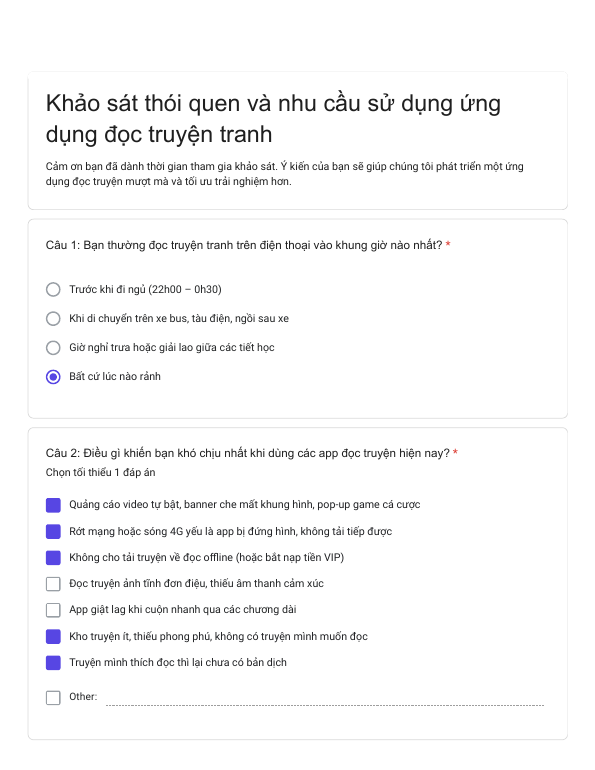
\includegraphics[width=0.95\textwidth,height=7.8cm,keepaspectratio]{figures/survey/p-01.png}}
        \caption{Survey Form -- Questions 1 \& 2 (Respondent 1)}
    \end{subfigure}
    \hfill
    \begin{subfigure}[b]{0.48\textwidth}
        \centering
        \fbox{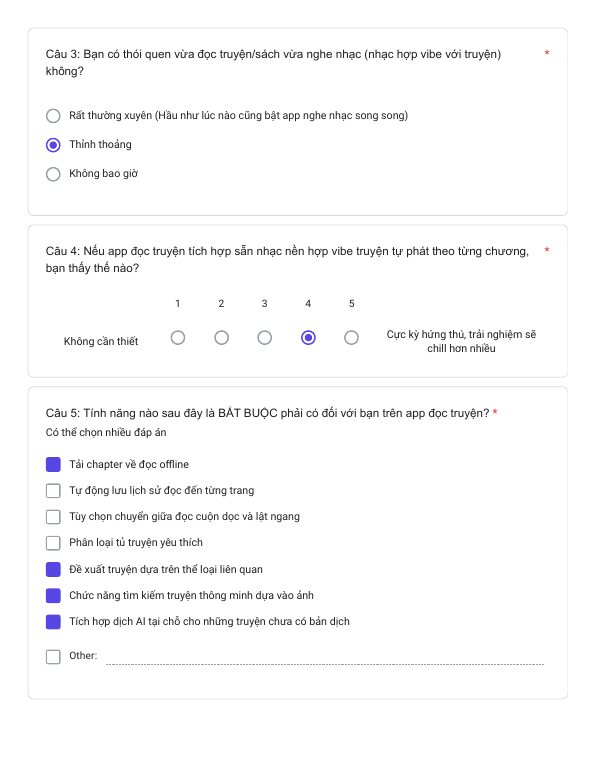
\includegraphics[width=0.95\textwidth,height=7.8cm,keepaspectratio]{figures/survey/p-02.png}}
        \caption{Survey Form -- Questions 3, 4 \& 5 (Respondent 1)}
    \end{subfigure}
    \caption{Sample empirical evidence extracted from the Google Forms user elicitation archive (\texttt{khao\_sat\_4\_nguoi.pdf}).}
    \label{fig:survey_evidence}
\end{figure}

\subsubsection{Quantitative Statistical Synthesis \& Architectural Implications}
Table~\ref{tab:survey_stats} consolidates the quantitative distribution of user pain points and feature demands alongside the concrete engineering decisions derived for \textbf{Naomi}.

\begin{table}[H]
\centering
\caption{Quantitative synthesis of elicitation findings and direct architectural implications.}
\label{tab:survey_stats}
\footnotesize
\renewcommand{\arraystretch}{1.25}
\begin{tabularx}{\textwidth}{L{4.2cm} C{2.0cm} Y}
\toprule
\rowcolor{tablehead}
\textbf{Empirical Finding / Metric} & \textbf{Prevalence} & \textbf{Direct Engineering \& Specification Decision} \\
\midrule
\textbf{Intrusive video/banner/gambling ads} (Q2) & \textbf{100.0\%} ($4/4$) & Strict \textbf{100\% Ad-Free commitment}; zero advertising or tracking SDKs; monetisation/IAP explicitly excluded as \texttt{WON'T-HAVE} (\texttt{FR-15}). \\
\rowcolor{tablerow}
\textbf{Habit of pairing music with reading} (Q3) \& \textbf{Ambient Audio Rating} (Q4) & \textbf{100.0\%} ($4/4$)\newline Mean: \textbf{3.75 / 5.0} & Core differentiator (\textbf{Unique Value Proposition}): integrate \texttt{just\_audio} streaming from Supabase Storage matched to comic genres (\texttt{FR-05}, \texttt{FR-09}, \texttt{UC-04}). \\
\textbf{Missing translations} (Q2) \& \textbf{In-place AI Translation demand} (Q5) & \textbf{75\%--100\%} ($3\text{--}4/4$) & Specify in-place AI chapter translation overlay (\texttt{FR-12}) on the Reader top toolbar (\texttt{S05} Icon $\star$) as a high-value \texttt{COULD-HAVE} capability. \\
\rowcolor{tablerow}
\textbf{Exact page-level reading history} (Q5) & \textbf{75.0\%} ($3/4$) & Persist \texttt{last\_page\_read} and \texttt{read\_percentage} asynchronously in SQLite ($\le 50\text{ ms}$) with bidirectional Supabase cloud sync (\texttt{FR-04}, \texttt{NFR-09}) and surface on the \texttt{S02} Home Hero card. \\
\textbf{Limited catalog} (Q2) \& \textbf{Genre-based recommendations} (Q5) & \textbf{75.0\%} ($3/4$) & Integrate the open \textbf{MangaDex REST API v5} catalog (\texttt{FR-01}, \texttt{FR-08}) with horizontal \textit{Trending} and \textit{Genre} discovery carousels (\texttt{S03}, \texttt{S03b}). \\
\rowcolor{tablerow}
\textbf{Cellular network freezes \& lack of free offline mode} (Q2, Q5) & \textbf{50.0\%} ($2/4$) & Design a \textbf{Hybrid Offline-First Architecture} with full-chapter pre-buffering (\texttt{S10}), 1-tap local chapter downloads (\texttt{FR-06}, \texttt{S11}), and $\le 300\text{ ms}$ offline fallback (\texttt{FR-13}, \texttt{S09} $\to$ \texttt{S07}). \\
\textbf{Scrolling lag on long chapters} (Q2) & \textbf{50.0\%} ($2/4$) & Enforce \textbf{60 FPS rendering} ($\le 16.6\text{ ms/frame}$, \texttt{NFR-03}) via Flutter Impeller/Skia virtualised viewport lists and strict file-system media storage (never storing image BLOBs in SQLite). \\
\rowcolor{tablerow}
\textbf{Visual image search from screenshots} (Q5) & \textbf{50.0\%} ($2/4$) & Provide camera icon trigger on \texttt{S03} invoking the OS \textbf{System Photo Picker} (\texttt{FR-11}), achieving visual search with \textbf{zero storage permissions} (\texttt{NFR-12}). \\
\textbf{Willingness to adopt Naomi over existing apps} (Q6) & \textbf{100.0\%} ($4/4$) & Validates strong product-market fit provided the core Must-Have and Should-Have baseline is delivered cleanly in Assignment 02. \\
\bottomrule
\end{tabularx}
\end{table}
